\documentclass[a4paper,10pt]{article}
\usepackage{enumitem}
\usepackage{titlesec}
\usepackage{geometry}
\usepackage{graphicx}
\geometry{margin=1in}

% Title Information
\title{\Huge \textbf{Spotify Documentation}}
\date{}

\begin{document}

% Cover Page
\begin{titlepage}
    \centering
    \vspace*{2cm}

    \vspace{1cm}
    \includegraphics[width=0.5\textwidth]{7124272_spotify_logo_icon.png}

    \vspace{1cm}
    \Huge
    \textbf{Software Engineering Project}

    \vspace{1cm}
    \LARGE
    To: Eng. Manar mukhlis.

    \vfill
    
    \Large
    \textbf{Team Members} \\
    Ahmed Ehab Ahmed Elsayid Elattar (G4 ID: 22030007) \\
    Ahmed Amin Soliman Amin (G4 ID: 22030004) \\
    Shahda Mohamed Abd Elkareem (G4 ID: 22030092) \\
    Menna Ahmed Abdel Mohsen (G4 ID: 2203018) \\
    Bassant Hossam Salah (G4 ID: 2203004) \\
    Salma Mohamed Gamal (G4 ID: 22030084) \\
    Habiba Mohamed Sayid (G4 ID: 22030049)

    \vspace{2cm}
\end{titlepage}

% Table of Contents
\newpage
\tableofcontents
\newpage

% Content Sections
\section{Introduction}
Music consumption was fundamentally changed with the rise of digital media. As technology advanced, the demand for instant, on-demand access to music grew. Before streaming, most people either bought CDs or downloaded individual songs. This setup was limited, expensive, and inconvenient in a rapidly digitalizing world.

\section{Problem Statement}
Consumers wanted a way to listen to a wide range of music instantly, without the high costs and hassle of purchasing individual songs or albums. Additionally, artists and the music industry needed a platform to combat piracy, which had surged as people sought free access to music.

\section{Solution}
Spotify was developed as a streaming platform offering affordable, unlimited access to a vast music library. By using an ad-supported model and offering subscriptions, Spotify could provide free and premium options, addressing consumer needs while compensating artists. This approach created a legal, accessible, and enjoyable way to consume music on demand.

\section{System Objective and Scope}
% Add content here

\section{Stakeholders}
    \subsection{Primary Stakeholders}
    These are the people who directly interact with and use the system. They are the main users whose needs and experiences are prioritized during the system's design and development.

    \begin{itemize}
        \item \textbf{Users:} The individuals who subscribe to and use Spotify to stream music, create playlists, and discover new content.
        \item \textbf{Admins:} The team members responsible for managing the platform’s operations, such as content moderation, user support, and system management.
    \end{itemize}

    \subsection{Secondary Stakeholders}
    These are individuals or entities that have an interest in the system but do not directly use it as primary stakeholders do. They may influence or be affected by the system in various ways.

    \begin{itemize}
        \item \textbf{Partners:} Record labels, artists, and content creators who provide music and other content for Spotify.
        \item \textbf{Banks and Financial Institutions:} These entities handle financial transactions and payments for subscriptions, royalties, and other financial operations.
        \item \textbf{Advertisers:} Companies that purchase advertising space within the Spotify app to reach its user base.
    \end{itemize}

\section{Motivation}
% Add content here

\section{User Requirements}
\subsection{1. User Characteristics}
    \begin{itemize}[leftmargin=*]
        \item \textbf{User ID and Username:} Each user must have a unique identifier and username to ensure distinct profiles and prevent duplication.
        \item \textbf{Age and Parental Controls:} The system will capture users’ ages and provide parental control options for younger users to monitor and manage accessible content.
        \item \textbf{Subscription and Payment Methods:} Users will have the option to select between free and premium subscriptions, with multiple flexible payment methods available.
        \item \textbf{Email and Contact Information:} Valid contact details, including email, are required for notifications and account recovery purposes.
        \item \textbf{Account Type:} Accounts will be categorized as either a regular User account or an Artist account, determining available features and functionalities.
    \end{itemize}

\subsection{2. Functional Requirements}
\subsubsection{2.1 User Management}
    \begin{itemize}[leftmargin=*]
        \item \textbf{Account Creation:} Users can register using email or phone, with an option for social media linked account sign-ins.
        \item \textbf{Profile Updates:} Users can update their profile information, including username, profile picture, and contact details.
        \item \textbf{Subscription Management:} Users can upgrade, downgrade, or cancel their subscriptions at any time, with corresponding feature adjustments.
        \item \textbf{Linked Accounts:} Users can link social media accounts to enhance connectivity and sharing options.
    \end{itemize}

\subsubsection{2.2 Music Streaming and Library Management}
    \begin{itemize}[leftmargin=*]
        \item \textbf{Music Streaming:} The system shall provide free (with ads) and premium (ad-free) streaming options, with users controlling playback based on their subscription type.
        \item \textbf{Personalized Playlists:} Curated playlists tailored to user preferences and listening history will be offered (e.g., “Top Hits,” “Discover Weekly”).
        \item \textbf{Playlist Management:} Users can create, edit, and delete playlists, as well as add or remove songs.
        \item \textbf{Advanced Search:} Users can search for music by artist, title, genre, mood, and keywords for easy content location.
    \end{itemize}

\subsubsection{2.3 Social and Sharing Features}
    \begin{itemize}[leftmargin=*]
        \item \textbf{Social Media Sharing:} Users can share playlists or songs on social media platforms through a visually appealing interface.
        \item \textbf{Follower and Following System:} Users can follow friends and artists to stay updated on new music and shared playlists.
        \item \textbf{Blending Feature:} Users can blend their music tastes with friends to explore common interests and discover new music.
        \item \textbf{Collaborative Playlists:} Users can co-create playlists with friends and listen together in real-time.
    \end{itemize}

\subsection{3. Non-Functional Requirements}
\subsubsection{3.1 Performance and Scalability}
    \begin{itemize}[leftmargin=*]
        \item \textbf{Load Time:} The system shall load songs within a maximum of 2 minutes to ensure a seamless user experience.
        \item \textbf{Search Query Performance:} The system shall efficiently handle a minimum of X concurrent search queries.
        \item \textbf{User Growth Management:} The system shall dynamically manage user growth to ensure consistent performance as the user base expands.
    \end{itemize}

\subsubsection{3.2 Usability and Accessibility}
    \begin{itemize}[leftmargin=*]
        \item \textbf{User Interface Design:} The system shall feature an intuitive and user-friendly interface that facilitates easy navigation for all users.
        \item \textbf{Accessibility Standards:} The application shall comply with established accessibility standards, making it usable for individuals with disabilities and supporting multiple languages.
    \end{itemize}

\subsubsection{3.3 Security and Compliance}
    \begin{itemize}[leftmargin=*]
        \item \textbf{Data Encryption:} Sensitive user data shall be encrypted both in transit and at rest to protect against unauthorized access.
        \item \textbf{Multi-Factor Authentication:} The system shall implement multi-factor authentication to enhance security during user login.
        \item \textbf{Legal Compliance:} The system shall comply with applicable data protection laws and regulations, including automatic protection measures and secure data backup protocols.
    \end{itemize}

\section{Similar Systems}
\subsection{Anghami}
Anghami is a music streaming service similar to Spotify, focused on the Middle Eastern and North African (MENA) region. Launched in 2012, it was the first legal music streaming service in the Arab world, tailored to local tastes and cultural preferences. It offers a vast library of Arabic and international music, podcasts, and personalized playlists. Like Spotify, Anghami allows users to stream music online or download it for offline listening, offering both free and premium subscription options. Anghami also integrates culturally relevant features, such as local charts, and often includes more regional content, making it popular among Arabic-speaking users.

\section{DFD - Context Diagram (Level 0)}
\begin{figure}[h!]
    \centering
    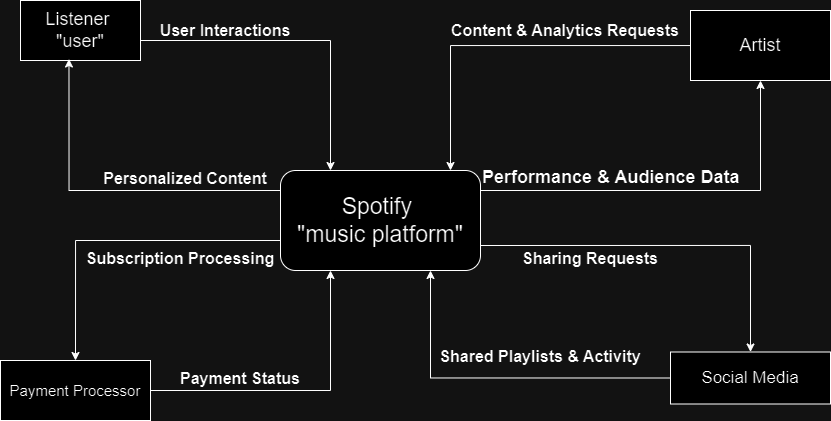
\includegraphics[width=0.8\textwidth]{DFD@Dark.drawio.png}
    \caption{DFD Level 0 - Context Diagram for Spotify-like Application}
    \label{fig:dfd-level0}
\end{figure}

\end{document}
